\documentclass{InsightArticle}

\usepackage[dvips]{graphicx}
\usepackage{float}
\usepackage{subfigure}

\usepackage[dvips,
bookmarks,
bookmarksopen,
backref,
colorlinks,linkcolor={blue},citecolor={blue},urlcolor={blue},
]{hyperref}


\title{A Conditional Mesh Front Iterator for VTK}

% 
% NOTE: This is the last number of the "handle" URL that 
% The Insight Journal assigns to your paper as part of the
% submission process. Please replace the number "1338" with
% the actual handle number that you get assigned.
%
\newcommand{\IJhandlerIDnumber}{3162}

% Increment the release number whenever significant changes are made.
% The author and/or editor can define 'significant' however they like.
\release{1.00}

% At minimum, give your name and an email address.  You can include a
% snail-mail address if you like.

\author{David Doria}
\authoraddress{Rensselaer Polytechnic Institute}


\begin{document}

%
% Add hyperlink to the web location and license of the paper.
% The argument of this command is the handler identifier given
% by the Insight Journal to this paper.
% 
\IJhandlefooter{\IJhandlerIDnumber}


\ifpdf
\else
   %
   % Commands for including Graphics when using latex
   % 
   \DeclareGraphicsExtensions{.eps,.jpg,.gif,.tiff,.bmp,.png}
   \DeclareGraphicsRule{.jpg}{eps}{.jpg.bb}{`convert #1 eps:-}
   \DeclareGraphicsRule{.gif}{eps}{.gif.bb}{`convert #1 eps:-}
   \DeclareGraphicsRule{.tiff}{eps}{.tiff.bb}{`convert #1 eps:-}
   \DeclareGraphicsRule{.bmp}{eps}{.bmp.bb}{`convert #1 eps:-}
   \DeclareGraphicsRule{.png}{eps}{.png.bb}{`convert #1 eps:-}
\fi


\maketitle

\ifhtml
\chapter*{Front Matter\label{front}}
\fi

\begin{abstract}
\noindent
Region growing is a technique that can be used to propagate information over a mesh. In a previous submission, ``A Mesh Front Iterator for VTK'', we introduced an iterator that can be used with $vtkPointSet$ subclasses to traverse a mesh. It is sometimes useful to visit only vertices that are ``similar'' to their neighbors by some definition. This concept can be used to select many types of common regions, including planar regions or regions with similar color, to name a few. In this paper, we propose an iterator which propagates on a mesh using a condition test which can be easily modified.
\end{abstract}

\IJhandlenote{\IJhandlerIDnumber}

\tableofcontents

%%%%%%%%%%%%%%%%%
\section{Introduction}
Region growing is a technique that can be used to propagate information over a mesh. In a previous submission, ``A Mesh Front Iterator for VTK'' (\verb|http://www.midasjournal.org/browse/publication/724|), we introduced an iterator that can be used with $vtkPointSet$ subclasses to traverse a mesh. It is sometimes useful to visit only vertices that are ``similar'' to their neighbors by some definition. This concept can be used to select many types of common regions, including planar regions (similar normals) or regions with similar color, to name a few. In this paper, we present an iterator which propagates on a mesh to regions which pass one or more conditional tests. We provide several such tests, and provide a simple abstract interface which can be used to implement custom comparison functions.

%%%%%%%%%%%%%%
\section{Algorithm}
Front propagation is essentially a breadth first search. The initial ``front'' is the set of immediate neighbors (connected by an edge) of the seed vertex. To propagate the front, we perform the procedure described below.

\subsection{Initialization}
\begin{itemize}
\item Add the seed vertex to a queue.
\end{itemize}

\subsection{Iteration}
\begin{itemize}
\item Get the vertex in the front of the queue. Set $NextId$ to this value.
\item Add all of the vertices that are connected to $NextId$ and pass all of the condition tests to the back of the queue, unless they have already been visited or are already in the queue.
\item Mark $NextId$ as visited.
\item Return $NextId$.
\end{itemize}

%%%%%%%%%%%%%%%
\section{Condition Interface}
An abstract $Condition$ class can be subclassed to provide any type of vertex comparison function.

The function which must be implemented to determine the comparison function is:
\begin{verbatim}
virtual bool IsSimilar(const int a, const int b) = 0;
\end{verbatim}

where $a$ and $b$ are the ids of two vertices. This function returns true if the comparison function determines that the two vertices are ``close enough'' to each other with the specified metric.

This comparison will always reference a mesh, which is set with:

\begin{verbatim}
void SetMesh(vtkPolyData* m) {this->Mesh = m;} 
\end{verbatim}

We suggest overriding this function in each subclass to ensure that the attributes on which the comparison function operates are present in the supplied mesh.
 
%%%%%%%%%%%%%%%
\section{Provided Conditions}
We have included several Condition subclasses for common comparison operations.

\subsection{NormalCondition}
This Condition should be used to detect planar regions, or gradually varying regions of a mesh. The \verb|AcceptableAngle| parameter controls how similar adjacent normals must be to be considered ``close enough'' to pass the test.

\subsection{ColorCondition}
This Condition should be used to regions of a mesh with similar colors. The \verb|AcceptableDifference| parameter controls how similar adjacent colors must be to be considered ``close enough'' to pass the test.

\subsection{DistanceCondition}
This Condition should be used to ``connected'' regions of a mesh. The \verb|AcceptableDistance| parameter controls how close  adjacent points must be to be considered ``close enough'' to pass the test.

%%%%%%%%%%%%%%
\section{Demonstration}

Figure \ref{fig:Demo} shows two selections on a typical LiDAR data set. Figure \ref{fig:scan} shows the input mesh. The green points in Figure \ref{fig:ground} shows how the ground can be selected by selecting a single seed point (the red point). Figure \ref{fig:wall} shows how unlike many ground detection algorithms (which rely on the ground plane having a normal of approximately $(0,0,1)$), this region growing approach is much more general and can also be used to select a wall. These examples use the \verb|vtkMeshNormalConditionFrontIterator| with the \verb|NormalCondition|.

\begin{figure}[H]
\centering
\subfigure[Input mesh]{
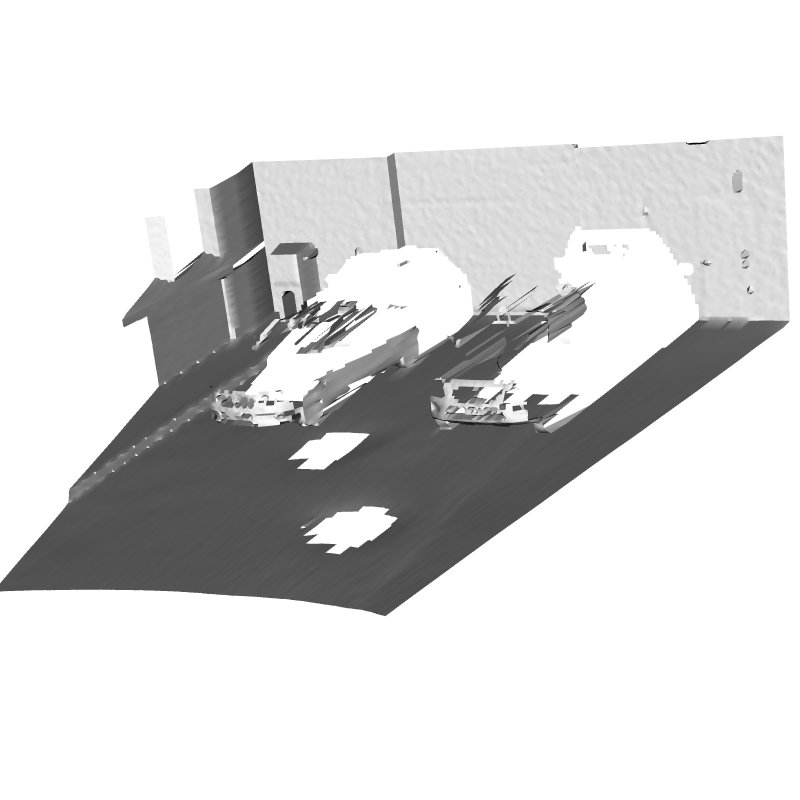
\includegraphics[width=0.3\linewidth]{Images/scan}
\label{fig:scan}
}
\subfigure[Selected ground]{
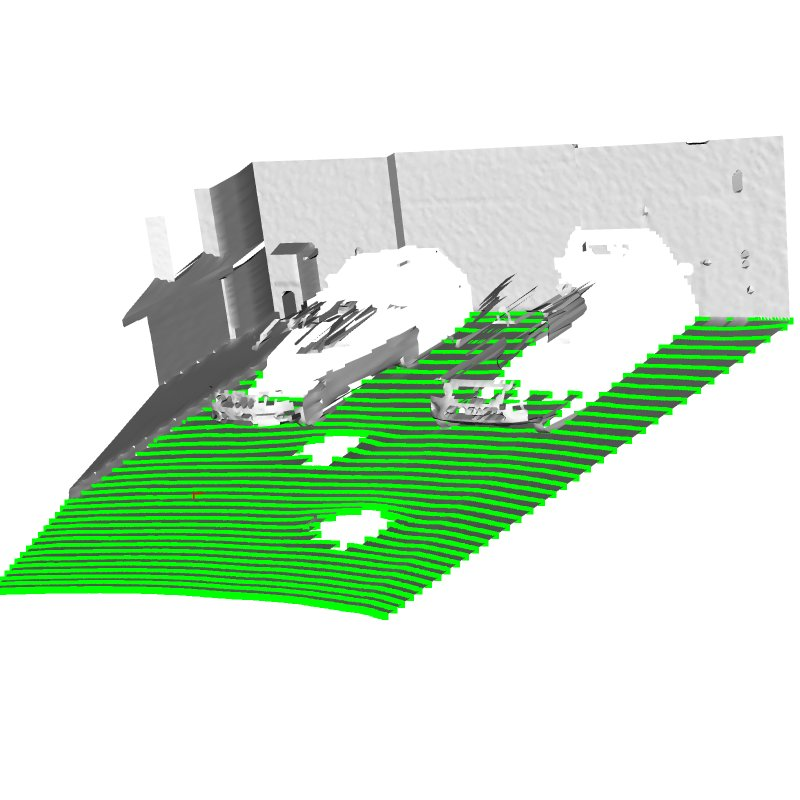
\includegraphics[width=0.3\linewidth]{Images/ground}
\label{fig:ground}
}
\subfigure[Selected wall]{
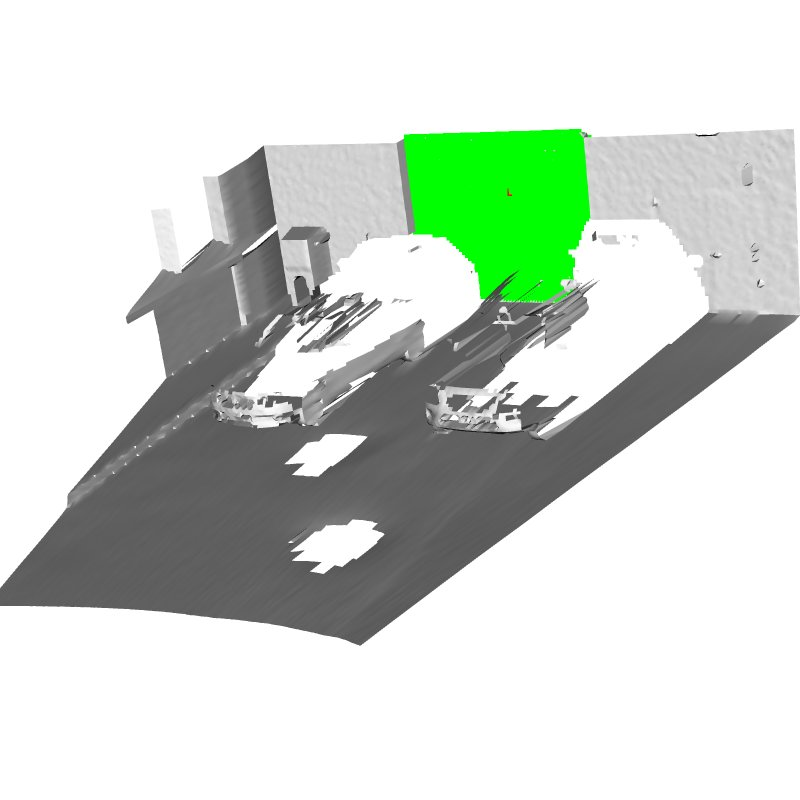
\includegraphics[width=0.3\linewidth]{Images/wall}
\label{fig:wall}
}
\caption{Demonstration of growing regions conditioned on normal similarity.}
\label{fig:Demo}
\end{figure}

%%%%%%%%%%%%%%
\section{Extracting the region that has been grown}

%%%%%%%%%%%%%%
\section{Code Snippet}
The interface is straight forward:

\begin{verbatim}
  DistanceCondition* condition = new DistanceCondition;
  condition->SetAcceptableDistance(1.);
    
  vtkSmartPointer<vtkMeshConditionalFrontIterator> iterator = 
    vtkSmartPointer<vtkMeshConditionalFrontIterator>::New();
  iterator->SetCondition(condition);
  iterator->SetMesh(normalsFilter->GetOutput());
  iterator->SetStartVertex(0);
  iterator->Initialize();

  // Inspect the order of the growing
  while(iterator->HasNext())
    {
    vtkIdType nextVertex = iterator->Next();
    std::cout << "Next vertex: " << nextVertex << std::endl;
    }

  // Extracted the region that was reached
  vtkSmartPointer<vtkPolyData> region = vtkSmartPointer<vtkPolyData>::New();
  iterator->GetSelectedRegion(region);

  // Mark the region that was reached by adding a membership array to the input mesh
  iterator->MarkSelectedRegion();

\end{verbatim}

Note that if all of the Conditions are not passed to the iterator before the \verb|vtkMeshConditionalFrontIterator::SetMesh| function is called, that the Conditions will not have access to the mesh unless the user had manually called \verb|SetMesh| on the condition directly.

\end{document}
